\documentclass[a4paper]{article}
\usepackage[utf8]{inputenc}
\usepackage[T1]{fontenc}
\usepackage[french]{babel}
\usepackage{amsmath,amsfonts,amssymb}
\usepackage{bookman}
\usepackage{xcolor}
\usepackage{array}
\usepackage{pifont}
\usepackage{ulem}
\usepackage{listings}
\usepackage{graphicx}
\usepackage{eurosym}
\usepackage[left=2cm, right=2cm, top=2cm, bottom=2cm]{geometry}
\frenchbsetup{StandardLists=true}
\newcommand\coord[3]{\begin{pmatrix}
#1 \\
#2 \\
#3
\end{pmatrix}}
\newcommand{\R}{\mathbb{R}}
\newcommand{\N}{\mathbb{N}}
\newcommand{\D}{\mathbb{D}}
\newcommand{\Z}{\mathbb{Z}}
\newcommand{\Q}{\mathbb{Q}}
\newcommand{\C}{\mathbb{C}}
\newcommand{\K}{\mathbb{K}}
\newcommand{\lra}{\Longrightarrow}
\newcommand{\lla}{\Longleftarrow}
\newcommand{\llra}{\Longleftrightarrow}
\setlength{\textheight}{23.5cm}
\newcommand{\ra}{\rightarrow}
\newcommand{\la}{\leftarrow}

\let\oldsection\section
\renewcommand{\section}[1]{\textcolor{purple}{\oldsection{#1}}}
\let\oldsubsection\subsection
\renewcommand{\subsection}[1]{\textcolor{cyan}{\oldsubsection{#1}}}
\let\oldsubsubsection\subsubsection
\renewcommand{\subsubsection}[1]{\textcolor{green}{\oldsubsubsection{#1}}}
\let\oldtextbf\textbf
\renewcommand{\textbf}[1]{\textcolor{cyan}{\oldtextbf{#1}}}
\let\oldunderline\underline
\renewcommand{\underline}[1]{\textcolor{purple}{\oldunderline{#1}}}
\let\oldtextit\textit
\renewcommand{\textit}[1]{\textcolor{violet}{\oldtextit{#1}}}

\lstset{
    inputencoding=utf8,
    extendedchars=true,
    literate=%
    {é}{{\'{e}}}1
    {è}{{\`{e}}}1
    {ê}{{\^{e}}}1
    {ë}{{\¨{e}}}1
    {û}{{\^{u}}}1
    {ù}{{\`{u}}}1
    {â}{{\^{a}}}1
    {à}{{\`{a}}}1
    {î}{{\^{i}}}1
    {ô}{{\^{o}}}1
    {ç}{{\c{c}}}1
    {Ç}{{\c{C}}}1
    {É}{{\'{E}}}1
    {Ê}{{\^{E}}}1
    {À}{{\`{A}}}1
    {Â}{{\^{A}}}1
    {Î}{{\^{I}}}1,
    basicstyle=\footnotesize\sffamily\color{black},
    commentstyle=\textcolor{gray},
    numbers=left,
    numbersep=5pt,
    numberstyle=\textcolor{gray},
    keywordstyle=\textcolor{teal},
    showspaces=false,
    showstringspaces=false,
    stringstyle=\textcolor{magenta},
    tabsize=2
}

\title{Time Bomb: Premier rapport}
\author{Ilias Deligiannis, Florent Weber, Nadjib Belaribi, Danyl El-Kabir,\\
Leonardo Nassabain, François Grabenstaetter}

\begin{document}
\sffamily
\everymath{\displaystyle}
\setlength\parindent{0mm}
\setlength{\parskip}{0.2cm}
\maketitle

\section{Menu et interfaces hors-partie}

\subsection{Accueil}

\begin{center}
    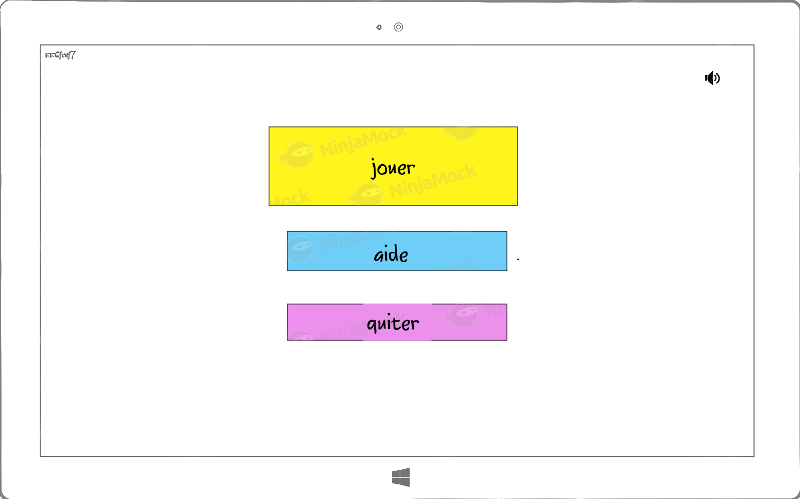
\includegraphics[scale=2]{img/accueil.png}
\end{center}

Le menu d'accueil, très simplifié, met en avant le \textit{bouton play}. Ainsi, les joueurs (qui sont là pour ça) peuvent commencer au plus vite à jouer.

Le choix de la langue a été placé de sorte qu'on ne puisse pas involontairement cliquer dessus.

\newpage
\subsection{Paramètres de partie}

\begin{center}
    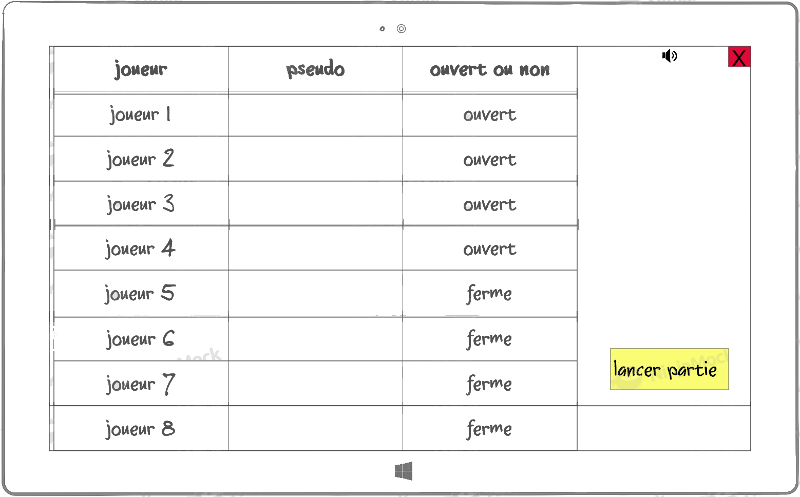
\includegraphics[scale=2]{img/param_partie.png}
\end{center}

Cette fenêtre nous permettra de définir le nombre de joueurs et leurs pseudo. Il suffit que chaque joueur saisisse un pseudo dans une zone de texte puis d'utiliser le bouton en bas à droite pour lancer la partie.

On aura donc autant de joueurs que de zones de texte remplies. Nous pensons qu'il s'agit d'un façon simple et facilement compréhensible pour les joueurs, de présenter les choses.

\subsection{Le tutoriel interactif}

On a voulu faire un tutoriel interactif qui ressemblera plus à une histoire racontée qu'à un simple tutoriel.

Puisqu'il s'agit d'un jeu de rôle avec deux camps bien définis, nous trouvons que transmettre les règles à travers \textit{un dialogue} entre Moriarty et Sherlock pourrait être plutôt sympa.

\subsection{La fin d'une partie}

Lorsqu'une partie de jeu se termine, une fenêtre affiche quelle est l'équipe gagnante et propose les choix \textit{replay}, \textit{menu} et \textit{desktop} pour quitter.

\begin{center}
    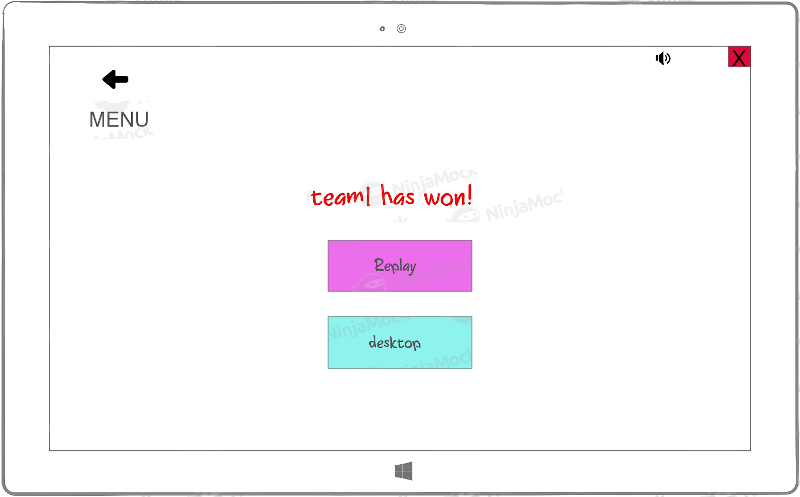
\includegraphics[scale=2]{img/ecran_fin_partie.png}
\end{center}

\section{Interface de la partie de jeu}

\subsection{État de jeu initial d'une manche}

\begin{center}
    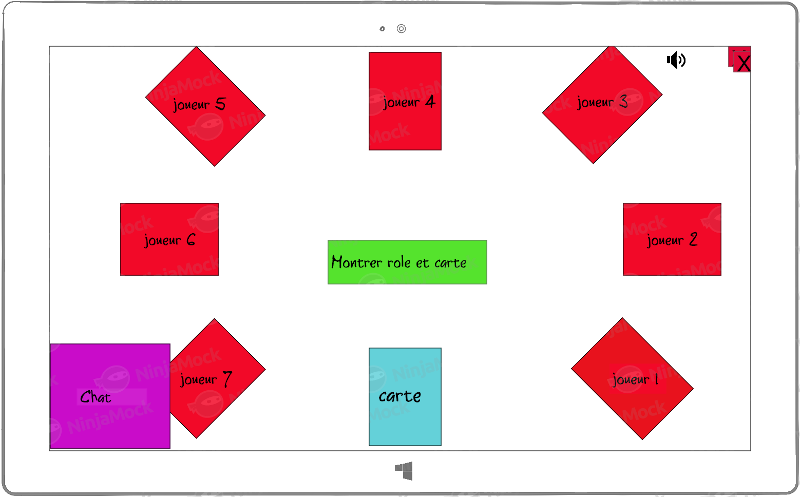
\includegraphics[scale=2]{img/partie_avant_devoiler.png}
\end{center}

Il s'agit de la fenêtre principale de jeu. Cependant, vu que le jeu se déroule en local (sur une seule machine pour tous les joueurs, pour le moment) il nous faut un moyen pour que les joueurs puissent prendre connaissance de leur rôle et cartes: appuyer sur le bouton au milieu (\textit{Montrer role et carte}) pour chaque joueur (chacun son tour), lorsqu'il est prêt (et que les autres ne regardent pas !)

Cette astuce nous permet de donner l'impression d'avoir ses propres cartes en partageant une seule machine. La prochaine wireframe affiche les cartes et le rôle du joueur en question:

\begin{center}
    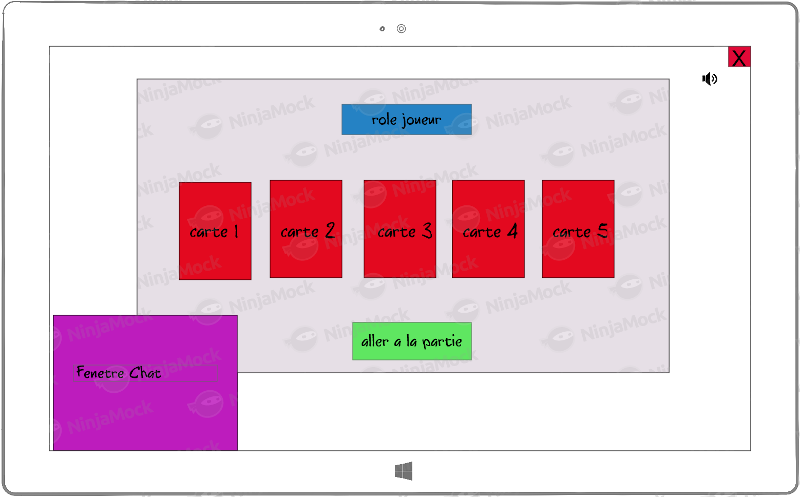
\includegraphics[scale=2]{img/decouvert_role_et_carte.png}
\end{center}

\subsection{État de jeu normal}

\begin{center}
    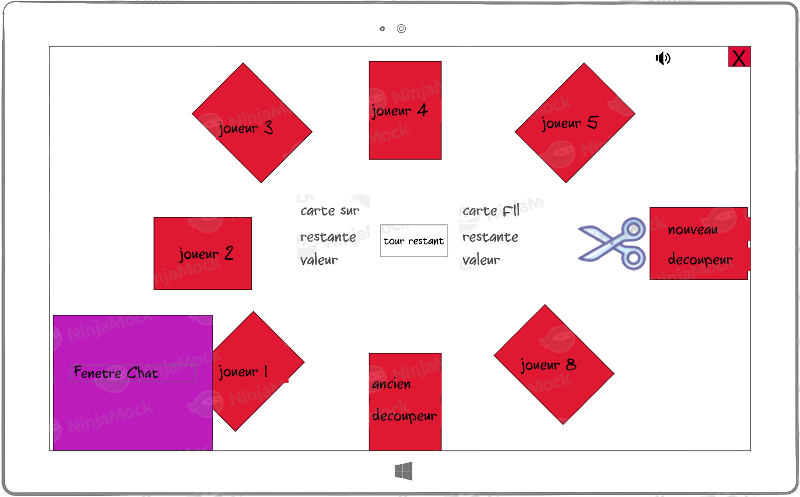
\includegraphics[scale=2]{img/ecran_partie_quand_joueur_pas_choix.png}
\end{center}

On représente ici la fenêtre dans l'état de jeu normal: le tour du joueur actuel est indiqué par la pince, ainsi que quelques informations bien visibles au milieu de l'écran (nombre de cartes sûres et dangereuses restantes, et le nombre de tours restants)

\subsection{Choix d'une carte à découper (action du joueur actuel)}

\begin{center}
    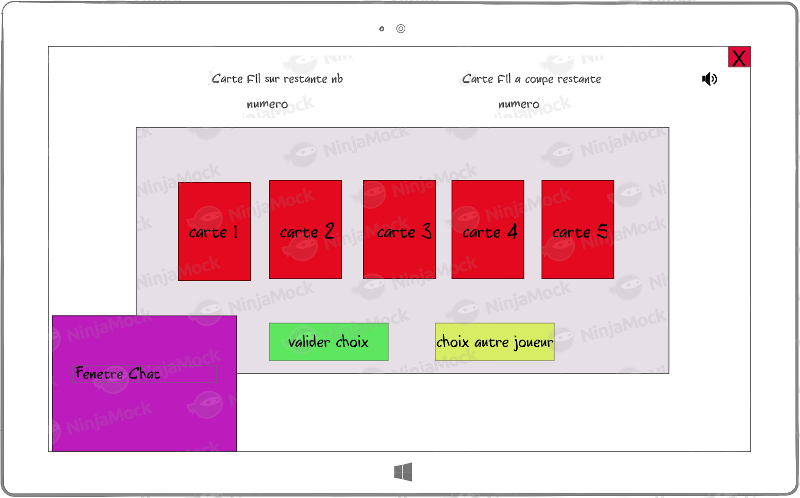
\includegraphics[scale=2]{img/choix_carte_a_defausser.png}
\end{center}

Cette fenêtre apparait lorsqu'un joueur doit découper une carte (à son tour). Il peut choisir une des cartes affichées pour un certain joueurs ou celles d'un autre joueur en cliquant sur le bouton \textit{choix autre joueur} puis valide avec le bouton \textit{valider choix}. Le nombre de cartes sûres restantes ainsi que celui des cartes dangereuses est affiché en haut afin que le joueur ne perde pas le fil de la partie.

\begin{center}
    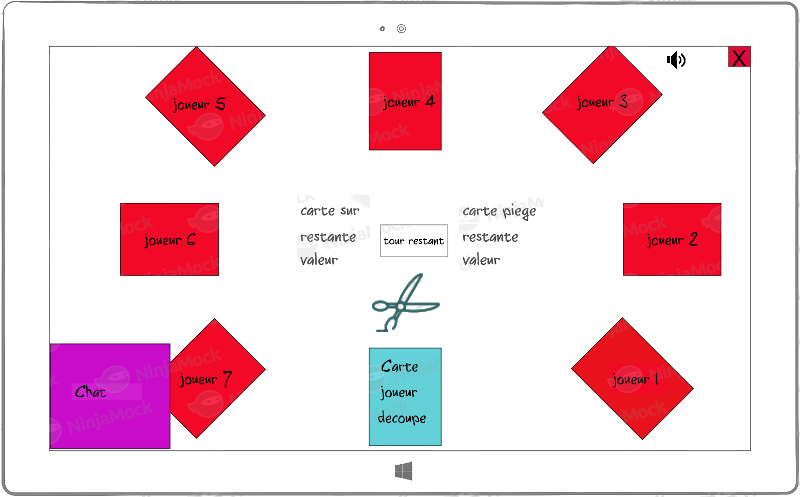
\includegraphics[scale=2]{img/choix_joueur_carte_defausse.png}
\end{center}

Après que le joueur ait choisit une carte à découper, elle s'affiche sur l'écran pour que tout le monde puisse la voir.

\end{document}
